To make use of the {\it \systemNameFull} you need to be able to assemble software programs 
for the {\processor} processor and then execute these programs in the computer system. There are 
two main approaches for getting started: using a simulation of the computer system, or
using an FPGA board that implements the computer system in hardware.

\subsubsection {Using the CPUlator Simulator}

The {\it CPUlator} is a powerful and easy-to-use functional simulator that runs inside a
web browser. It simulates the behavior of a whole computer system, including the
processor, memory, and many types of I/O devices. The CPUlator simulator supports a variety
of different computer systems, including the {\it \systemNameFull}. 

The CPUlator user interface displays all of the information that a programmer needs to
develop and debug software code running on the {\it \systemNameFull}. It shows (and allows
you to edit) the values in the processor general-purpose and control registers, as well as the 
contents of memories in the computer system and the values of memory-mapped I/O device 
registers. The CPUlator allows software code, written either in assembly language or the 
C language, to be entered into the simulator, assembled to produce machine code, loaded 
into memory, and then executed. The user can set breakpoints in the machine code, 
single-step instructions, and perform any of the usual operations that are supported in 
typical debugging environments. A screen capture of the CPUlator user interface is shown 
in Figure~\ref{fig:CPUlator}. It displays the processor registers on the 
left-hand side (by default) of the screen,
the program code in the middle, and graphical representations of I/O devices on the 
right-hand side.

\begin{figure}[h!]
   \begin{center}
        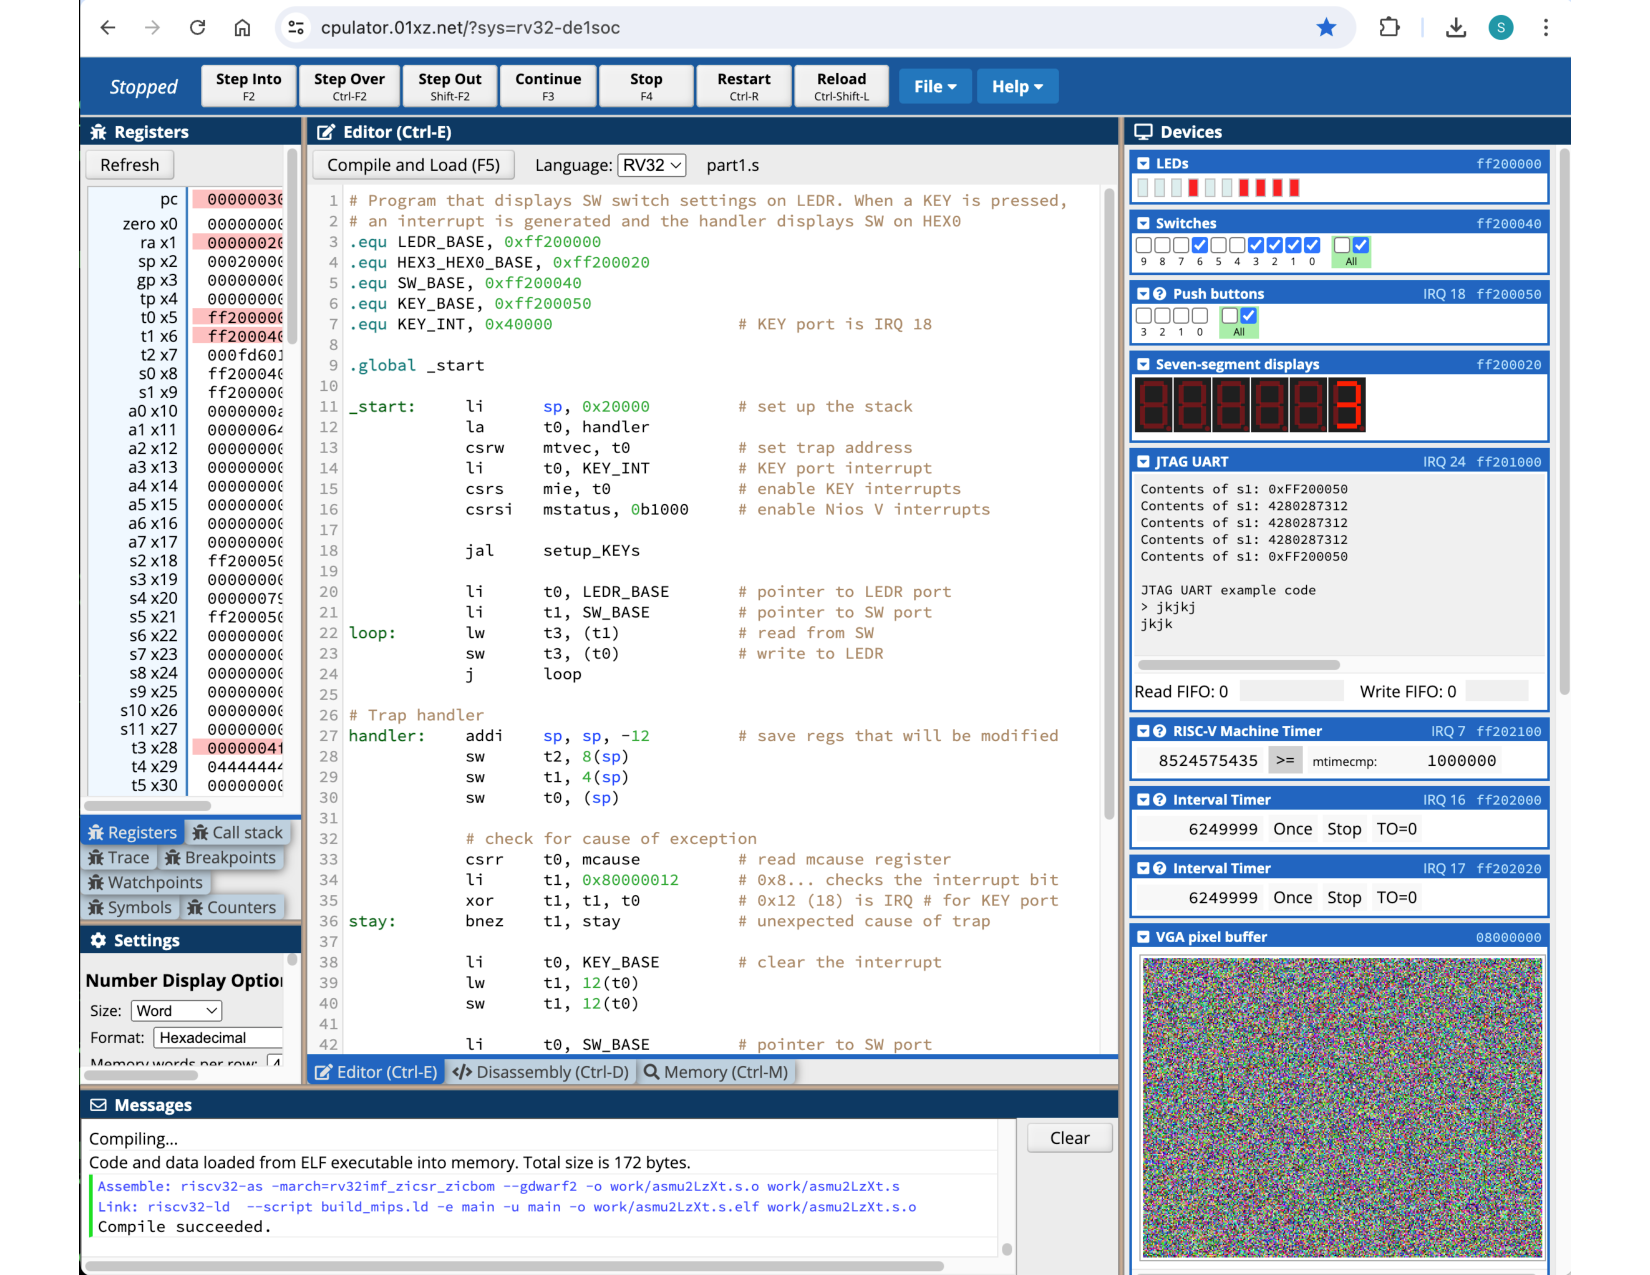
\includegraphics[scale=.66]{figures/CPUlator.pdf}
   \end{center}
   \caption{The CPUlator.}
	\label{fig:CPUlator}
\end{figure}

\subsubsection {Using the {\productNameMed{}} with an FPGA Hardware Board}

The {\it \systemNameFull} can be implemented using a {\DEBoard} hardware
board.  An easy way to begin working with this computer system 
is to make use of the utility called the {\it \productNameMed{}}.  It
provides an easy way to assemble/compile {\processor} programs 
written in either assembly language or the C language. The Monitor 
Program, which can be downloaded from the \texttt{Software Tools} section of the
\href{https://www.fpgacademy.org/tools.html} {FPGAcademy.org} website,
is an application program that 
runs on the host computer connected to the \DEBoard~board.  The Monitor Program can be 
used to control
the execution of code on {\processor}, list (and edit) the contents of processor registers, 
display/edit the contents of memory on the \DEBoard~board, and similar operations.
The Monitor Program includes the \systemName~as a pre-designed system that can be
downloaded onto the \DEBoard~board, as well as several sample programs in assembly language and
C that show how to use the {\it \systemNameFull} peripheral devices.
Some images that show how the {\it \systemNameFull} is integrated with the 
Monitor Program are given in Section~\ref{sec:monitor_program}.
An overview of the Monitor Program is available in the document
{\it \productNameMed{} Tutorial for the {\processor} Processor}, which is provided 
as part of the \texttt{Computer Organization System Design} tutorials on
\href{https://www.fpgacademy.org/tutorials.html} {FPGAcademy.org}.

\subsubsection {Using GDB with an FPGA Hardware Board}
The {\it \productNameMed{}} controls the FPGA hardware and the {\processor}
processor by using the industry-standard GNU Project Debugger ({\it GDB}). Instead of using
the {\it \productNameMed{}}, you can debug code with the {\it GDB} tool directly.
%A tutorial that shows how to use {\it GDB} with the {\it \systemNameFull}
%is available on \href{https://www.fpgacademy.org/tutorials.html} {FPGAcademy.org}.
